\subsection{Incast}
\label{incast}


%%% incast, 16 to 1 %%%
% see , /power/home/keq/workloads/program/acdctcp/incast-container16-10Minutes
\begin{table*}[!htb]
\begin{center}
\begin{tabular}{ |c|c|c|c|c|c| }
 \hline
  & Avg Tput (Mbps) & Fairness Index & 50$^{th}$ percentile TCP RTT ($\mu$s) & 99.9$^{th}$ percentile TCP RTT ($\mu$s) & Drop Rate \\
 \hline

 Default & 619 & 0.98 & 3607 & 11599 & 0.14\% \\
 DCTCP  & 619 & 0.99 & 197 & 486 & 0 \\
 Ours & 598 & 0.99 &  93 & 289 & 0 \\
 \hline
\end{tabular}
\caption{16 to 1 incast test. MTU = 9000 B. Marking min = 10.}
\label{incast_16to1_tbl_9000}
\end{center}
\end{table*}

%see, /power/home/keq/workloads/program/acdctcp/marking_tune
\iffalse
\begin{table*}[!htb]
\begin{center}
\begin{tabular}{ |c|c|c|c|c|c| }
 \hline
  & Avg Tput (Mbps) & Fairness Index & 50$^{th}$ percentile TCP RTT ($\mu$s) & 99.9$^{th}$ percentile TCP RTT ($\mu$s) & Drop Rate \\
 \hline

 Default & 619 & 0.98 & 3585 & 4022 & 0.14\% \\
 DCTCP  & 618 & 0.99 & 195 & 543 & 0 \\
 Ours & 610 & 0.98 &  120 & 456 & 0 \\
 \hline
\end{tabular}
\caption{16 to 1 incast test. MTU = 9000 B. Marking min = 99.}
\label{incast_16to1_tbl_9000_markingMin99}
\end{center}
\end{table*}
\fi
%see, /power/home/keq/workloads/program/acdctcp/incast-container32-10Minutes
\begin{table*}[!htb]
\begin{center}
\begin{tabular}{ |c|c|c|c|c|c| }
 \hline
  & Avg Tput (Mbps) & Fairness Index & 50$^{th}$ percentile TCP RTT ($\mu$s) & 99.9$^{th}$ percentile TCP RTT ($\mu$s) & Drop Rate \\
 \hline

 Default & 318 & 0.97 & 3729 & 14448 & 0.37\% \\
 DCTCP  & 319 & 0.99 & 448 & 792 & 0 \\
 Ours & 303 & 0.99 &  103 & 249 & 0 \\
 \hline
\end{tabular}
\caption{32 to 1 incast test. MTU = 9000 B. Marking min = 10.}
\label{incast_32to1_tbl_9000_markingMin10}
\end{center}
\end{table*}

%see, /power/home/keq/workloads/program/acdctcp/incast-container41
\begin{table*}[!htb]
\begin{center}
\begin{tabular}{ |c|c|c|c|c|c| }
 \hline
  & Avg Tput (Mbps) & Fairness Index & 50$^{th}$ percentile TCP RTT ($\mu$s) & 99.9$^{th}$ percentile TCP RTT ($\mu$s) & Drop Rate \\
 \hline

 Default & 245 & 0.96 & 3767 & 14596 & 0.55\% \\
 DCTCP  & 247 & 0.99 & 589 & 973 & 0 \\
 Ours & 238 & 0.99 &  130 & 327 & 0 \\
 \hline
\end{tabular}
\caption{40 to 1 incast test. MTU = 9000 B. Marking min = 10.}
\label{incast_40to1_tbl_9000_markingMin10}
\end{center}
\end{table*}


%see, /power/home/keq/workloads/program/acdctcp/incast-container48
\begin{table*}[!htb]
\begin{center}
\begin{tabular}{ |c|c|c|c|c|c| }
 \hline
  & Avg Tput (Mbps) & Fairness Index & 50$^{th}$ percentile TCP RTT ($\mu$s) & 99.9$^{th}$ percentile TCP RTT ($\mu$s) & Drop Rate \\
 \hline

 Default & 210 & 0.98 & 3792 & 15776 & 0.71\% \\
 DCTCP  & 210 & 0.99 & 684 & 1000 & 0 \\
 Ours & 201 & 0.99 &  121 & 314 & 0 \\
 \hline
\end{tabular}
\caption{47 to 1 incast test. MTU = 9000 B. Marking min = 10.}
\label{incast_47to1_tbl_9000_markingMin10}
\end{center}
\end{table*}



%%%%%%%%%%1500 bytes %%%%%%%%%%%%
\iffalse
%see, keq@arldcn26:~/workloads/program/acdctcp/incast-container16-10Minutes
\begin{table*}[!htb]
\begin{center}
\begin{tabular}{ |c|c|c|c|c|c| }
 \hline
  & Avg Tput (Mbps) & Fairness Index & 50$^{th}$ percentile TCP RTT ($\mu$s) & 99.9$^{th}$ percentile TCP RTT ($\mu$s) & Drop Rate \\
 \hline

 Default & 577 & 0.91 & 3073 & 3672 & 0.06\% \\
 DCTCP  & 451 & 0.97 & 312 & 707 & 0 \\
 Ours & 451 & 0.97 &  269 & 508 & 0 \\
 \hline
\end{tabular}
\caption{16 to 1 incast test. MTU = 1500 B. Marking min = 10.}
\label{incast_16to1_tbl_1500}
\end{center}
\end{table*}

%see, /power/home/keq/workloads/program/acdctcp/incast-container32-10Minutes
\begin{table*}[!htb]
\begin{center}
\begin{tabular}{ |c|c|c|c|c|c| }
 \hline
  & Avg Tput (Mbps) & Fairness Index & 50$^{th}$ percentile TCP RTT ($\mu$s) & 99.9$^{th}$ percentile TCP RTT ($\mu$s) & Drop Rate \\
 \hline

 Default & 294 & 0.96 & 3214 & 3702 & 0.08\% \\
 DCTCP  & 195 & 0.99 & 590 & 1080 & 0 \\
 Ours & 192 & 0.99 &  567 & 1035 & 0 \\
 \hline
\end{tabular}
\caption{32 to 1 incast test. MTU = 1500 B. Marking min = 10.}
\label{incast_32to1_tbl_1500_markingMin10}
\end{center}
\end{table*}

%see, /power/home/keq/workloads/program/acdctcp/incast-container41
\begin{table*}[!htb]
\begin{center}
\begin{tabular}{ |c|c|c|c|c|c| }
 \hline
  & Avg Tput (Mbps) & Fairness Index & 50$^{th}$ percentile TCP RTT ($\mu$s) & 99.9$^{th}$ percentile TCP RTT ($\mu$s) & Drop Rate \\
 \hline

 Default & 244 & 0.88 & 3221 & 4317 & 0.14\% \\
 DCTCP  & 154 & 0.99 & 834 & 1356 & 0 \\
 Ours & 154 & 0.99 &  807 & 1302 & 0 \\
 \hline
\end{tabular}
\caption{40 to 1 incast test. MTU = 1500 B. Marking min = 10.}
\label{incast_40to1_tbl_1500_markingMin10}
\end{center}
\end{table*}


%see, /power/home/keq/workloads/program/acdctcp/incast-container48
\begin{table*}[!htb]
\begin{center}
\begin{tabular}{ |c|c|c|c|c|c| }
 \hline
  & Avg Tput (Mbps) & Fairness Index & 50$^{th}$ percentile TCP RTT ($\mu$s) & 99.9$^{th}$ percentile TCP RTT ($\mu$s) & Drop Rate \\
 \hline

 Default & 202 & 0.93 & 3304 & 5049 & 0.12\% \\
 DCTCP  & 129 & 0.99 & 813 & 1396 & 0 \\
 Ours & 129 & 0.99 &  903 & 1438 & 0 \\
 \hline
\end{tabular}
\caption{47 to 1 incast test. MTU = 1500 B. Marking min = 10.}
\label{incast_47to1_tbl_1500_markingMin10}
\end{center}
\end{table*}

\fi
%%%%%%%%%%using figures to present incast: tput, fariness, droprate, TCP RTT
\begin{figure}[t]
        \centering
        \begin{subfigure}[b]{0.225\textwidth}
                \centering
                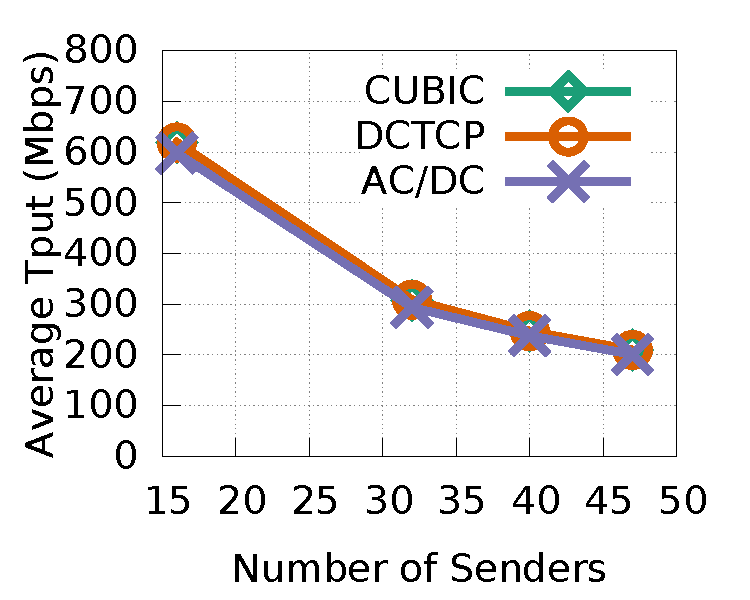
\includegraphics[width=\textwidth]{figures/incast/plots9k/incast_tput_vary_sender.pdf}
                \caption{average throughput}
                \label{incast_9k_tput}
        \end{subfigure}
        \begin{subfigure}[b]{0.225\textwidth}
                \centering
                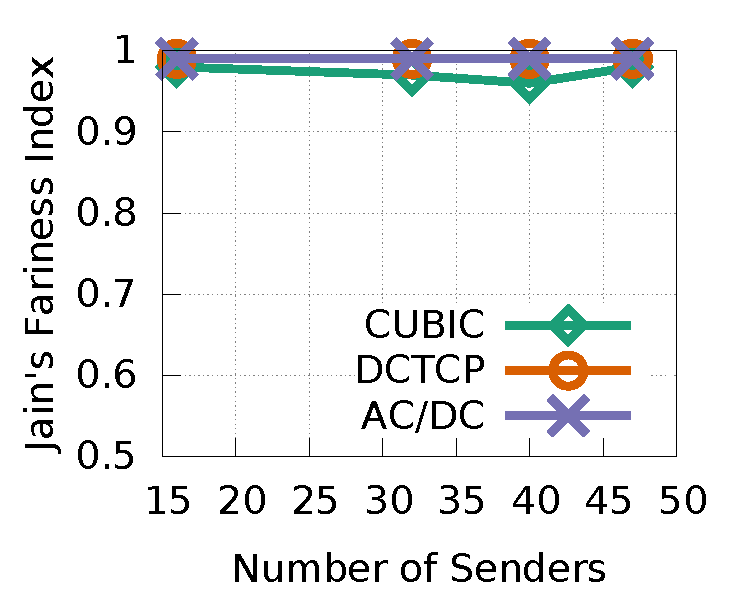
\includegraphics[width=\textwidth]{figures/incast/plots9k/incast_fairness_vary_sender.pdf}
                \caption{fairness}
                \label{incast_9k_fariness}
        \end{subfigure}
        \caption{Many to one incast: throughput and fairness.}
        \label{incast_9k_tput_fairness}
\end{figure}

\iffalse
\begin{figure}[t]
        \centering
        \begin{subfigure}[b]{0.225\textwidth}
                \centering
                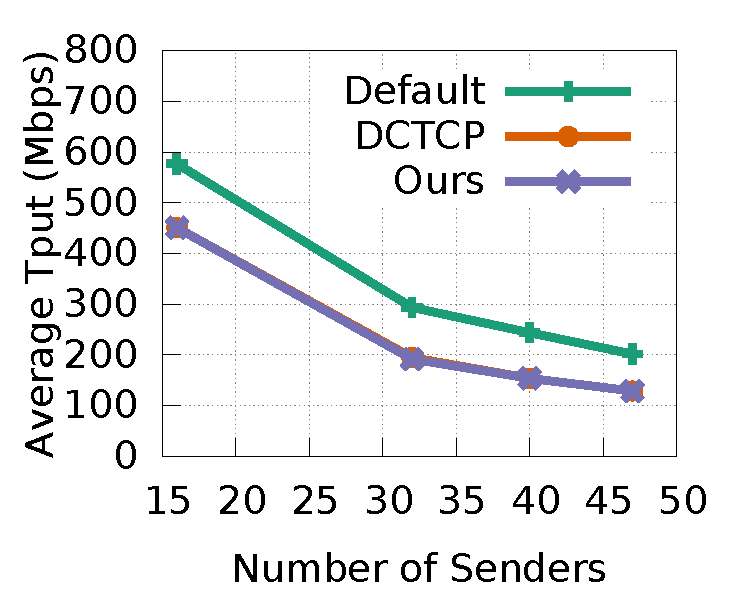
\includegraphics[width=\textwidth]{figures/incast/plots15k/15k_incast_tput_vary_sender.pdf}
                \caption{average throughput}
                \label{incast_15k_tput}
        \end{subfigure}
        \begin{subfigure}[b]{0.225\textwidth}
                \centering
                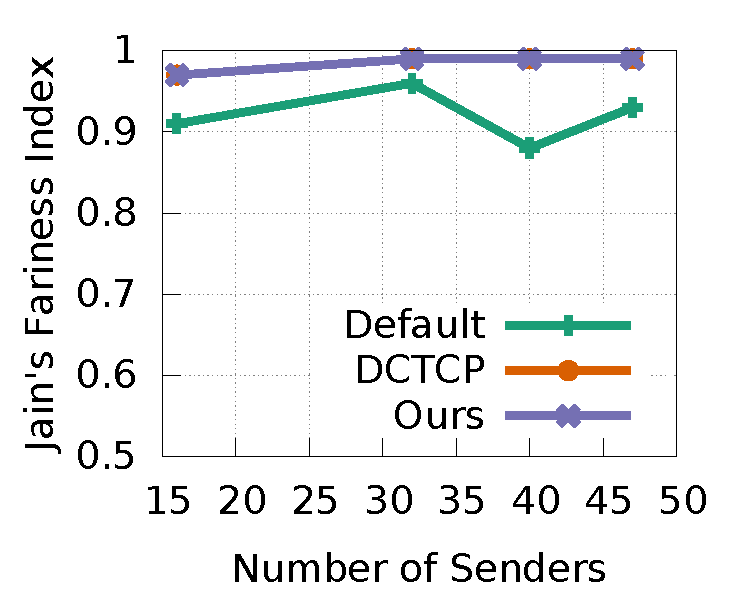
\includegraphics[width=\textwidth]{figures/incast/plots15k/15k_incast_fairness_vary_sender.pdf}
                \caption{fairness}
                \label{incast_15k_fariness}
        \end{subfigure}
        \caption{Incast, vary the number of sender. 1500Bytes.}
        \label{incast_15k_tput_fairness}
\end{figure}
\fi

\begin{figure*}[t]
        \centering
        \begin{subfigure}[b]{0.33\textwidth}
                \centering
                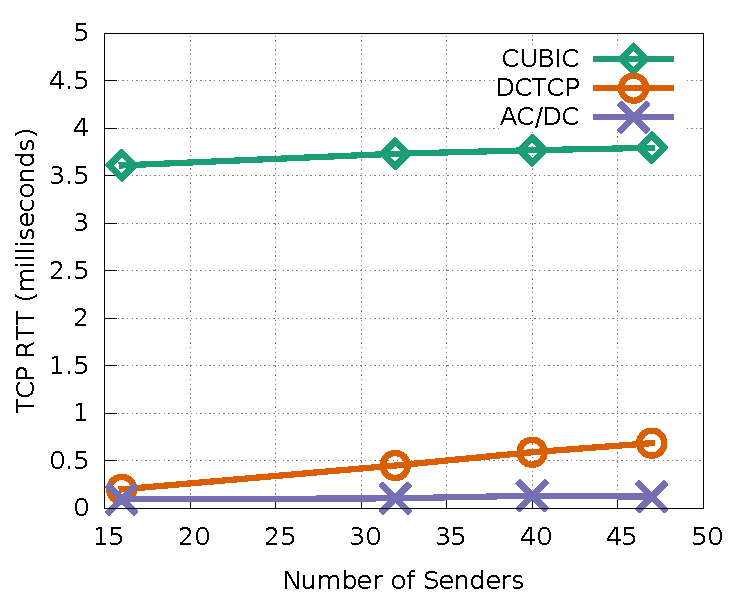
\includegraphics[width=\textwidth]{figures/incast/plots9k/incast_sockperf50th_vary_sender.pdf}
                \caption{50$^{th}$ percentile TCP RTT ($\mu$s).}
                \label{incast_9k_50th_sockperf}
        \end{subfigure}
        \begin{subfigure}[b]{0.33\textwidth}
                \centering
                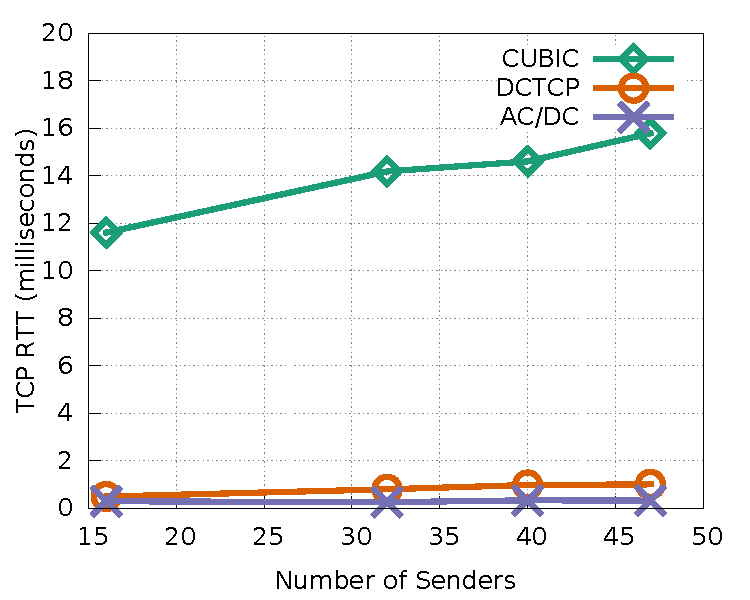
\includegraphics[width=\textwidth]{figures/incast/plots9k/incast_sockperf999th_vary_sender.pdf}
                \caption{99.9$^{th}$ percentile TCP RTT ($\mu$s).}
                \label{incast_9k_999th_sockperf}
        \end{subfigure}
        \begin{subfigure}[b]{0.33\textwidth}
                \centering
                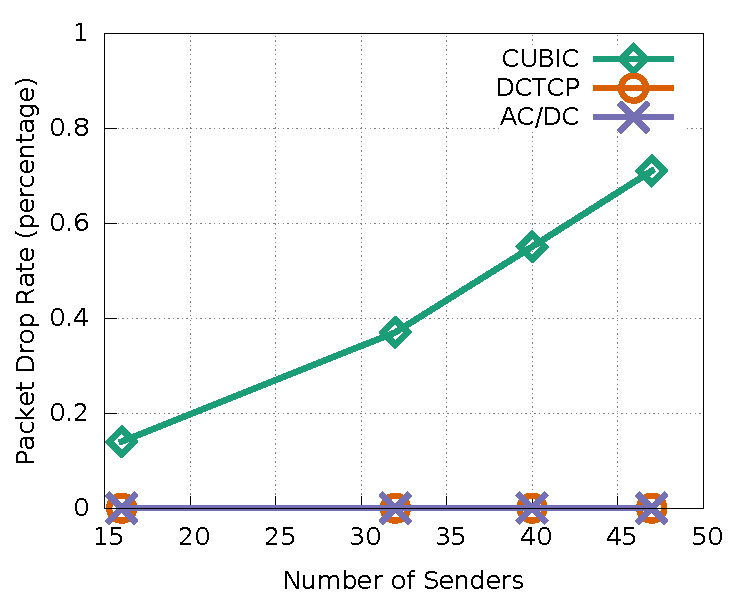
\includegraphics[width=\textwidth]{figures/incast/plots9k/incast_droprate_vary_sender.pdf}
                \caption{packet drop rate.}
                \label{incast_9k_droprate}
        \end{subfigure}
	\caption{Many to one incast: TCP RTT and packet drop rate.}
	\label{incast_9k_sockperf_droprate}
\end{figure*}

\iffalse
\begin{figure*}[t]
        \centering
        \begin{subfigure}[b]{0.33\textwidth}
                \centering
                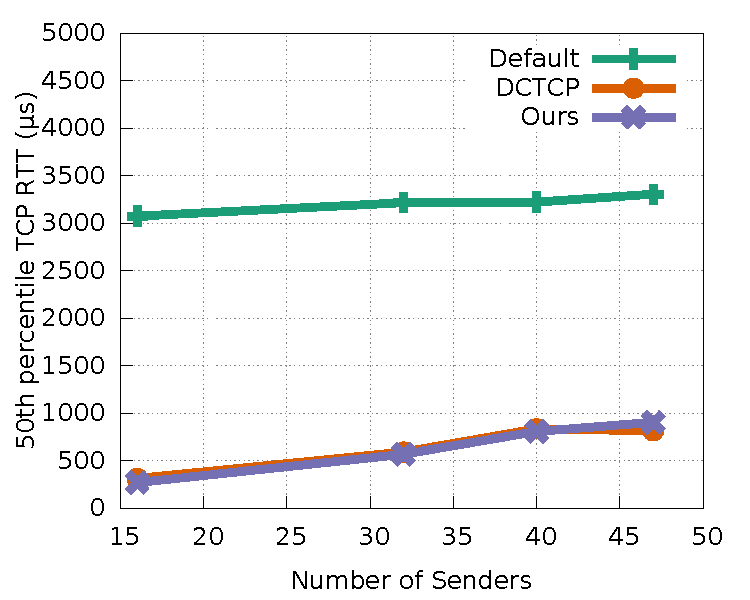
\includegraphics[width=\textwidth]{figures/incast/plots15k/15k_incast_sockperf50th_vary_sender.pdf}
                \caption{50$^{th}$ percentile TCP RTT ($\mu$s).}
                \label{incast_15k_50th_sockperf}
        \end{subfigure}
        \begin{subfigure}[b]{0.33\textwidth}
                \centering
                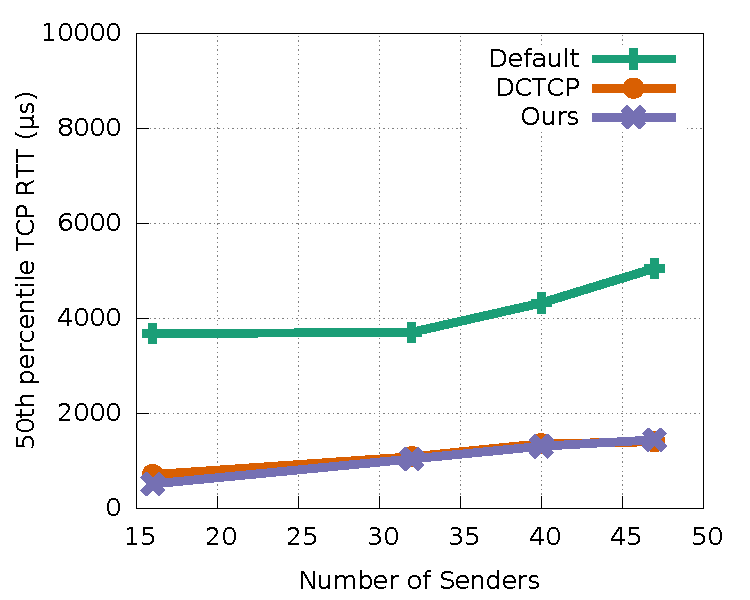
\includegraphics[width=\textwidth]{figures/incast/plots15k/15k_incast_sockperf999th_vary_sender.pdf}
                \caption{99.9$^{th}$ percentile TCP RTT ($\mu$s).}
                \label{incast_15k_999th_sockperf}
        \end{subfigure}
        \begin{subfigure}[b]{0.33\textwidth}
                \centering
                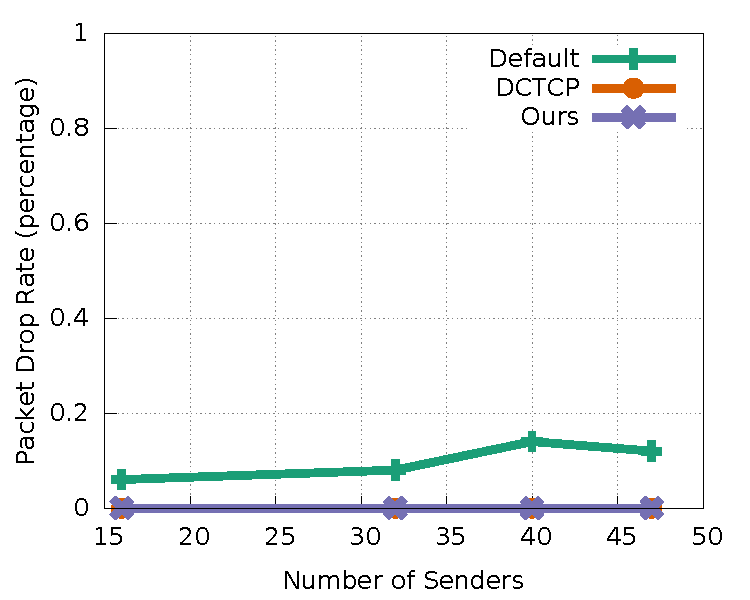
\includegraphics[width=\textwidth]{figures/incast/plots15k/15k_incast_droprate_vary_sender.pdf}
                \caption{packet drop rate.}
                \label{incast_15k_droprate}
        \end{subfigure}
        \caption{Incast. Vary the number of sender: 16, 32, 40 and 47. 1500 Bytes.}
        \label{incast_15k_sockperf_droprate}
\end{figure*}
\fi

%%%%47 to 1 incast, sockperf CDF %%%
\begin{figure}[t]
        \centering
  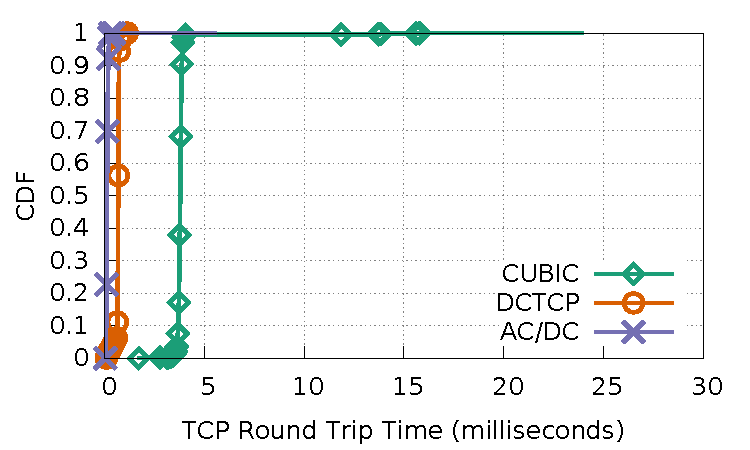
\includegraphics[width=0.45\textwidth]{figures/incast/47to1/incast_47to1_test_sockperf.pdf}
        \caption{TCP RTT in 47 to 1 incast test. MTU = 9000B.}
        \label{sockperf_incast_47to1}
\end{figure}

\begin{figure}[t]
        \centering
  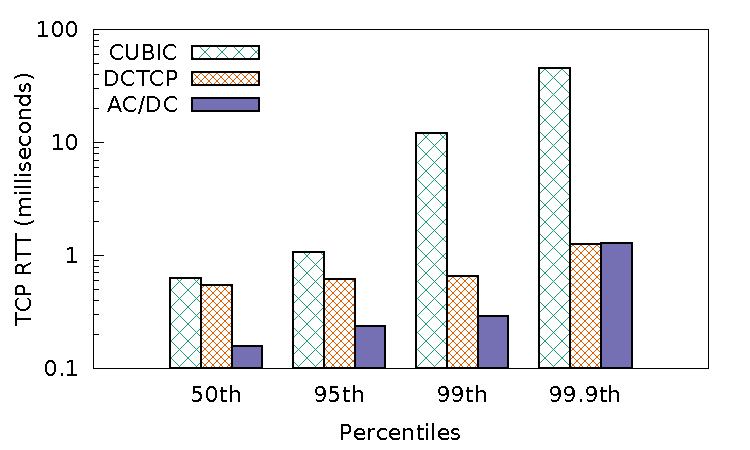
\includegraphics[width=0.45\textwidth]{figures/incast/pressure/incast_pressure_compare_sockperf.pdf}
        \caption{We want to check the case when almost every port of the switch is congested.
		We split 48 containers into 2 groups. 
		Each of the 46 containers in group A sends and receives 4 concurrent flows, 
		meanwhile, everyone in group A starts 1 flow to one container (denote as B1) 
		in group B to create 46 to 1 incast. TCP RTT is measured from B2 to B1.
		47 out of 48 ports are congested. MTU=9000. Average throughput for Default, 
		DCTCP, and Ours are 214, 214 and 201Mbps respectively, all with a fairness
		index greater than 0.98. Note that y-axis is in logscale. Default has an average 
		packet drop rate of 0.34\% but the most congested port has a drop rate of 4\%.}
        \label{sockperf_pressure_incast}
\end{figure}


In this section, we evaluate LiquidSwitch's performance in incast scenarios. 
For each experiment (i.e., each setting), we run it for 10 minutes.

\tightparagraph{Many to one}
First we test how \acdc{} performs in many to one incast. 
We have 17 physical servers in the testbed and each server has 4 NIC interfaces. 
To utilize all of the NIC interfaces, 
we set up Linux containers and let each container use one interface on the server. 
In this way, we can scale the number of instances to 68. 
We connect 48 containers to the switch such that all of 48 10Gbps ports on the switch are utilized. 
Then we gradually increase of extent of incast (number of concurrent senders is 16, 32, 40 and 47). 
Figure~\ref{incast_9k_sockperf_droprate} shows TCP RTT and packet drop rate results.
Figure~\ref{sockperf_incast_47to1} shows TCP RTT CDF in 47 to 1 incast. 
When there are 47 concurrent senders, DCTCP can reduce median TCP RTT by 82\% and \acdc{} can reduce by 97\%; 
DCTCP can reduce 99.9\%th percentile TCP RTT by 94\% and \acdc{} can reduce by 98\%; 
both DCTCP and \acdc{} get 0\% packet drop rate. \acdc{}’s performance is better than DCTCP, 
especially when the number of senders increases, The reason is that 
Linux DCTCP code (as well as the Stanford implementation)
puts a lower bound (which is 2) on CWND value. 
In the many to one incast test, we have up to 47 concurrent competing flows and
the network's MTU size is 9KB. In this case,
the lower bound of CWND can not reduce queue occupancy further.
So DCTCP's TCP increases gradually when the number of concurrent senders increases. 
This issue was also mentioned by~\cite{judd2015nsdi}.
In our scheme, we control RWND (which is in bytes) instead of CWND (which is in packets).
RWND's lowest value can be much smaller than 2*MSS.
So we can reduce the throughput further.
We checked that if we also put a lower bound, then our TCP RTT will be increased too.
Furthermore, controlling RWND is more fine-grained.
Figure~\ref{incast_9k_tput_fairness} shows TCP throughput and fairness results.
Both DCTCP and \acdc{} gets comparable throughput as Default and both offer a fairness index greater than 0.99\%.

\tightparagraph{All ports are congested}
